% Created 2016-04-08 fre 09:13
% Intended LaTeX compiler: pdflatex
\documentclass{scrartcl}
\usepackage[utf8]{inputenc}
\usepackage[T1]{fontenc}
\usepackage{graphicx}
\usepackage{grffile}
\usepackage{longtable}
\usepackage{wrapfig}
\usepackage{rotating}
\usepackage[normalem]{ulem}
\usepackage{amsmath}
\usepackage{textcomp}
\usepackage{amssymb}
\usepackage{capt-of}
\usepackage{hyperref}
\usepackage{khpreamble}
\author{Kjartan Halvorsen}
\date{2016-04-06}
\title{Computerized control - Partial exam 2 (20\%)}
\hypersetup{
 pdfauthor={Kjartan Halvorsen},
 pdftitle={Computerized control - Partial exam 2 (20\%)},
 pdfkeywords={},
 pdfsubject={},
 pdfcreator={Emacs 24.5.1 (Org mode 8.3.4)}, 
 pdflang={English}}
\begin{document}

\maketitle

\section*{Instructions}
\label{sec:orgheadline1}
\begin{itemize}
\item The exam is a take-home exam scheduled from Wednesday 2016-04-06 12:00 to Thursday 2016-04-07 23:59.
\item Write your answers clearly and motivate well! You can write by hand or on a computer. If you write by hand, you may scan your pages using, for instance, the app CamScanner that can produce pdf-documents.
\item You are allowed to talk to your fellow students about concepts in the course, about problem solving in general, and about the particular problems in the exam. \textbf{You are, however, not allowed to show or share partial or complete solutions to the problems.}
\item For acute questions, I can be reached by WhatsApp: 55 62 19 4048
\end{itemize}

\section*{Problem 1 RST-design}
\label{sec:orgheadline4}
The plant in figure \ref{fig:2dof} is described by the pulse-transfer function
\begin{equation}
H(z) = \frac{0.8}{z(z-0.8)},
\end{equation}
which is a first order system followed by a time-delay of one sampling period.

Let the desired characteristic polynomial of the closed-loop system be
\begin{equation}
A_{cl}(z) = \underbrace{z(z-0.7)}_{A_c(z)}\underbrace{(z-0.5)}_{A_o(z)}.
\end{equation}

\subsection*{(a) 40p}
\label{sec:orgheadline2}
Determine the polynomials \(R(z)\), \(S(z)\) and \(T(z)\) in an RST controller of the form in figure \ref{fig:2dof}. The pulse transfer function of the closed-loop system from the command signal \(u_c\) to \(y\) should be 
\begin{equation}
H_{c}(z) = \frac{0.3}{z(z-0.7)}.
\end{equation}
\begin{figure}
\begin{center}
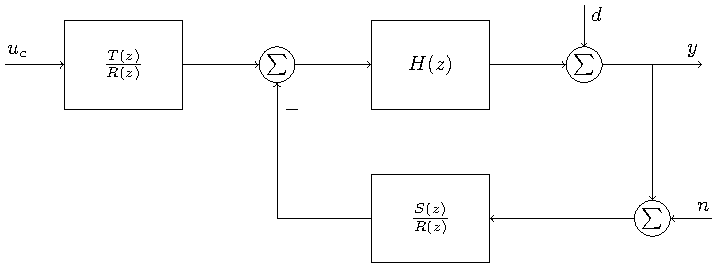
\includegraphics[width=0.7\linewidth]{../../homework/rst-block}
\caption{RST controller}
\label{fig:2dof}
\end{center}
\end{figure}

\subsection*{(b) 10p}
\label{sec:orgheadline3}
\begin{enumerate}
\item Calculate the pulse transfer function \(H_d(z)\) from the disturbance signal \(d\) to the output \(y\) for the closed-loop system using the controller you designed in (a).
\item Use matlab to calculate a response to a step in the disturbance \(d\). This can be done in a few lines:
\begin{verbatim}
num = % Your code here
den = % Your code here
Hd =  tf(num, den, -1); % Discrete-time system, undetermined sampling period
step(Hd)
\end{verbatim}
Include the step-response in your solution.
\item Bonus question (will give +5 points if correct, but no subtracted points if not correct): Why is the disturbance not eliminated by our control system? Hint: \(H_d(z)\) has \(R(z)\) as factor in the numerator. How could a \(R\) - polynomial suppress the step/constant disturbance?
\end{enumerate}

\section*{Problem 2 Discretization}
\label{sec:orgheadline7}
Consider the PD-controller
\begin{equation}
F(s) = 1 + \frac{s}{1 + \frac{s}{20}}.
\label{eq:pd}
\end{equation}

\subsection*{(a) 10p}
\label{sec:orgheadline5}
Determine a discrete-time controller \(F_d(z)\) using forward difference approximation (Euler's approximation).

\subsection*{(b) 20p}
\label{sec:orgheadline6}
\begin{enumerate}
\item What are the poles and zeros of the discrete-time controller?
\item For which values of the sampling time \(h>0\) is the discrete-time controller stable?
\end{enumerate}

\section*{Problem 3 Sampling and time-delay 20p}
\label{sec:orgheadline8}
A discrete-time controller involves sample-and-hold of the input signal to the controller. The sample-and-hold can be modelled as the transfer function (see Å\&W eq 7.27) 
\begin{equation}
G_{zoh}(s) = \frac{1}{s} \left( 1 - \mexp{-sh} \right).
\end{equation}
This block gives, approximately, a delay of half the sampling period, i.e. 
\begin{equation}
G_{zoh} (s) \approx h \mexp{-\frac{h}{2}s}.
\end{equation}

Choose  \(h=0.AB\), where \(AB\) are the last two digit of your matricula. Use matlab to generate the Bode diagrams of both \(G_{zoh}(s)\) and its approximation.

To help you get started, here is some code.
\begin{verbatim}
s = tf('s');
h = 0.62; % Use your own last two digits here!

G_zoh = 1/s * (1 - exp(-h * s) )
G_approx =   % Your code

figure(1)
clf
bode(G_zoh, G_approx, logspace(-1, log10(10*2*pi/h), 500));
legend('Sample-and-hold', 'Approximation', 'Location', 'Best')
\end{verbatim}

\begin{enumerate}
\item What is the Nyquist frequency?
\item Motivate why the approximation is reasonable for freqencies up to the Nyquist frequency (2-3 sentences).
\item Include the Bode diagram in your answer.
\end{enumerate}

\section*{Solutions}
\label{sec:orgheadline16}
\subsection*{Problem 1}
\label{sec:orgheadline11}
\subsubsection*{(a)}
\label{sec:orgheadline9}

The Diophantine equation
\[ A(z)R(z) + B(z)S(z) = A_c(z)A_o(z) \]
becomes
\[ \underbrace{z(z-0.8)}_{\text{order } 2}R(z) + \underbrace{0.8}_{\text{order } 0} S(z) = \underbrace{z^3-1.2z^2+0.35z }_{\text{order } 3}, \]
It is clear that to obtain the desired characteristic polynomial on the right hand side of the equation, we must choose a first-order controller:
\begin{align*}
R(z) &= z + r_1\\
S(z) &= s_0z + s_1.
\end{align*}
This gives the Diophantine equation
\[ z^3 + (r1 - 0.8)z^2 - 0.8r1z + 0.8s_0z + 0.8s_1 = z^3-1.2z^2+0.35z, \]
which gives the three equations 
\begin{align*}
r_1 -0.8 &= -1.2\\
-0.8r_1 + 0.8s_0 &= 0.35\\
0.8s1 &= 0,
\end{align*}
with solution
\begin{align*}
r_1  &= -0.4\\
s_0 &= 0.0375\\
s_1 &= 0.
\end{align*}

The pulse transfer function from \(u_c\) to \(y\) is 
\begin{equation*}
 \begin{split}
 H_c(z) &= \frac{\frac{T}{R}\frac{B}{A}}{1 + \frac{B}{A}\frac{S}{R}}\\
        &= \frac{TB}{AR+BS} = \frac{TB}{A_cA_o}.
 \end{split}
\end{equation*}
The polynomial \(T(z)\) is chosen to cancel the observer pole, so we have
\[ T(z) = t_0 A_o(z)\]
and
\[ H_c(z) = \frac{t_0B(z)}{A_c{z}} = \frac{0.8t_0}{z(z-0.7)}. \]
The  latter expression should be equal to 
\[ \frac{0.3}{z(z-0.7)}, \]
So,
\[t_0 = 0.3/0.8 = 0.375. \]

In summary, the controller is given by the three polynomials
\begin{align*}
R(z) &= z+r_1 = z-0.4\\
S(z) &= s_0z + s_1 = 0.0375z\\
T(z) &= t_0A_o(z) = 0.375(z - 0.5).
\end{align*}
\subsubsection*{(b)}
\label{sec:orgheadline10}
\begin{enumerate}
\item The pulse transfer function from \(d\) to \(y\) is given by
\begin{equation*}
 \begin{split}
  H_d &= \frac{1}{1 + \frac{B}{A}\frac{S}{R}} = \frac{AR}{AR + BS}\\
    &= \frac{z(z-0.8)(z-0.4)}{z(z-0.7)(z-0.5)}.
 \end{split}
\end{equation*}
\item The importance of the zeros of a pulse transfer function is that signals with frequency corresponding to the zeros will be blocked by the pulse transfer function. In order to eliminate the step disturbance, the corresponding frequency 
\[ \omega=0 \;\Rightarrow\; z=\mexp{i0h} = 1\]
should be a zero of the pulse transfer function \(H_d(z)\). In the RST-controller of figure \ref{fig:2dof}, the zeros of \(H_d\) are the roots of \(A(z)R(z)\). So, in order to eliminate the step disturbance, we must have at least one integration (pole in \(z=1\)) either in the plant \(\frac{B}{A}\) or in the controller \(\frac{S}{R}\).
\end{enumerate}

\subsection*{Problem 2}
\label{sec:orgheadline14}

\subsubsection*{(a)}
\label{sec:orgheadline12}
Euler's approximation of the differentiation operator is
\[ p \approx \frac{q-1}{h}. \]
This gives the approximate discrete PD-controller
\begin{equation*}
 \begin{split}
 F_d(z) &= F(s)|_{s = \frac{z-1}{h}} = 1 + \frac{\frac{z-1}{h}}{1 + \frac{z-1}{h}/20}\\
 &= 1 + \frac{20(z-1)}{20h + z - 1}\\
 &= \frac{z + 20h - 1 + 20z - 20}{z - (1-20h)}\\
 &= \frac{21z - (21 - 20h)}{z - (1-20h)}.
 \end{split}
\end{equation*}

\subsubsection*{(b)}
\label{sec:orgheadline13}
\begin{enumerate}
\item The pole is \(z_p=1-20h\) and the zero is \(z_z = \frac{21-20h}{21}\).
\item For the controller to be stable, the pole must be inside the unit circle. The pole is real, so we have
\[ -1 < 1-20h < 1. \]
Since \(h>0\), it is the lower inequality that we need to worry about. This gives
\[ 1-20h > -1 \quad \Rightarrow \quad h < 0.1. \]
\end{enumerate}

\subsection*{Problem 3}
\label{sec:orgheadline15}
\begin{enumerate}
\item The Nyquist frequency is 
\[ \omega_N = \frac{\pi}{h}. \]
\item With \(h=0.62\), I obtained the Bode-diagram in figure \ref{fig:bode}. Clearly, the phase plots (lower graph), which tells us about the delay in the filter, are not possible to distinguish for frequencies upto the Nyquist frequency. So the approximation is giving the correct delay. On the other hand, the magnitude differs significantly for frequencies that approach the Nyquist frequency. The approximation is a pure time-delay that does not change the magnitude of the signals, but the sample-and-hold circuit attenuates the signals.
\item See figure \ref{fig:bode}
\end{enumerate}

\begin{figure}
\begin{center}
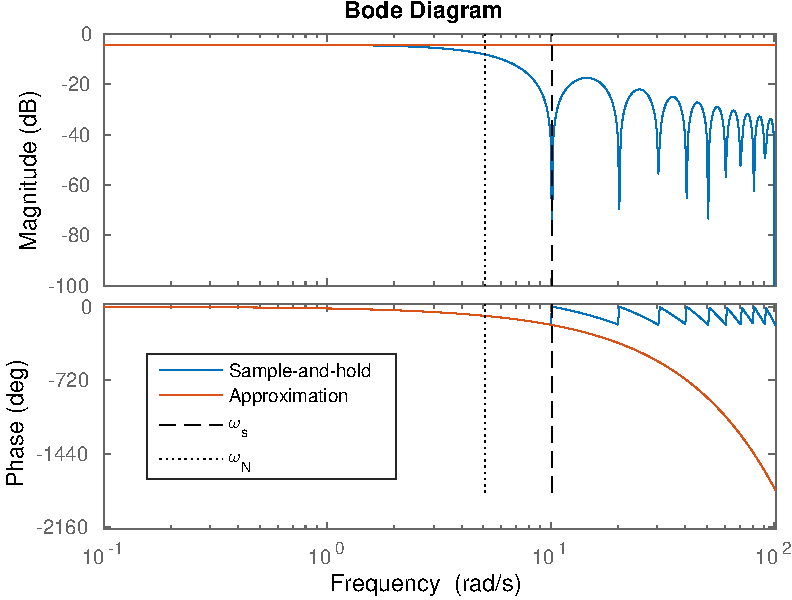
\includegraphics[width=0.7\linewidth]{bode-crop}
\caption{Bode-diagram of sample-and-hold circuit and of approximation}
\label{fig:bode}
\end{center}
\end{figure}
\end{document}
